\chapter{Results}
\label{results}

We generate and evaluate \textbf{3908 trajectories} using our evaluation methodology across all models. We make publicly available every trajectory alongside their corresponding overthinking score and the reasoning behind this score.

Our analysis reveals three key findings about overthinking in language models: its relationship with performance in SWE-bench, its non-equal prevalence across model types, and its practical implications for model selection. We observed that overthinking consistently impacts performance across all evaluated models, with reasoning-optimized models showing higher overthinking tendencies than general-purpose ones.

\section{Overthinking and Performance}
\label{sec:perf}

We anticipated that overthinking should impact performance as if models rely too heavily on their internal reasoning chain, there is a high likelihood that they will propose fixes based on inaccurate claims.

We observed a strong negative correlation between overthinking and performance on SWE-bench, as illustrated in \cref{fig:figure1}. Both reasoning and non-reasoning models show decreased performance as overthinking increases, though with notably different patterns.

\section{Overthinking and Model Type}
\label{sec:model_type}

We make three key observations with regards to overthinking in reasoning and non-reasoning models:

\subsection{Non-reasoning Models Can Overthink}
This observation can be explained by the presence of reasoning capabilities in non-reasoning models which could lead to overthinking. Recent studies show that non-reasoning models could have reasoning capabilities \cite{wei2023chainofthoughtpromptingelicitsreasoning, yao2023treethoughtsdeliberateproblem, chen2023program, kojima2023largelanguagemodelszeroshot}.

\subsection{Higher Overthinking in Reasoning Models}
Reasoning models significantly have higher overthinking scores compared to non-reasoning models, as shown in \cref{tab:overthinking_scores}. Since these models are specifically trained to reason and generate extended chains of thought by simulating environment interaction, they are more likely to suffer from manifestations of overthinking.

\subsection{Severe Impact on Non-reasoning Models}
Non-reasoning models that overthink suffer from severe degradation in issue resolution, as evidenced by the beta coefficients shown in \cref{tab:regression_results}. Lower beta coefficients indicate higher impact of overthinking on performance. We suspect that since non-reasoning models are not trained for reasoning, they are not capable of handling reasoning chains effectively, thus showing worse results.

\begin{table}[ht]
\centering
\begin{tabular}{lcccc}
\toprule
\textbf{Model} & \boldmath{$\beta_1$} & \boldmath{$R^2$} & \textbf{p-value} \\
\midrule
Reasoning      & -11.476 & 0.808 & 0.006 \\
Non-Reasoning  & -25.802 & 0.727 & 0.031 \\
\bottomrule
\end{tabular}
\caption{Regression Results for Reasoning and Non-Reasoning Models}
\label{tab:regression_results}
\end{table}

\begin{table}[ht]
\centering
\begin{tabular}{lc}
\toprule
\textbf{Measure} & \textbf{Value} \\
\midrule
Reasoning Models       & 2.320 $\pm$ 1.120 \\
Non-Reasoning Models   & 0.865 $\pm$ 0.432 \\
\midrule
T-test p-value         & 0.019 \\
\bottomrule
\end{tabular}
\caption{Average Overthinking Scores for Reasoning and Non-Reasoning Models}
\label{tab:overthinking_scores}
\end{table}

\section{Overthinking and Model Size}
\label{sec:model_size}

We analyzed two model families across four size variants (32B, 14B, 7B, and 1.5B): the non-reasoning Qwen2.5-Instruct \cite{qwen2,qwen2.5} and the reasoning R1-Distill-Qwen \cite{deepseekai2025deepseekr1incentivizingreasoningcapability}. Our analysis revealed two key patterns:

\begin{enumerate}
    \item Larger models demonstrate less tendency to overthink
    \item The gap in overthinking scores between reasoning and non-reasoning models widens at smaller scales
\end{enumerate}

\begin{figure}[t]
    \centering
    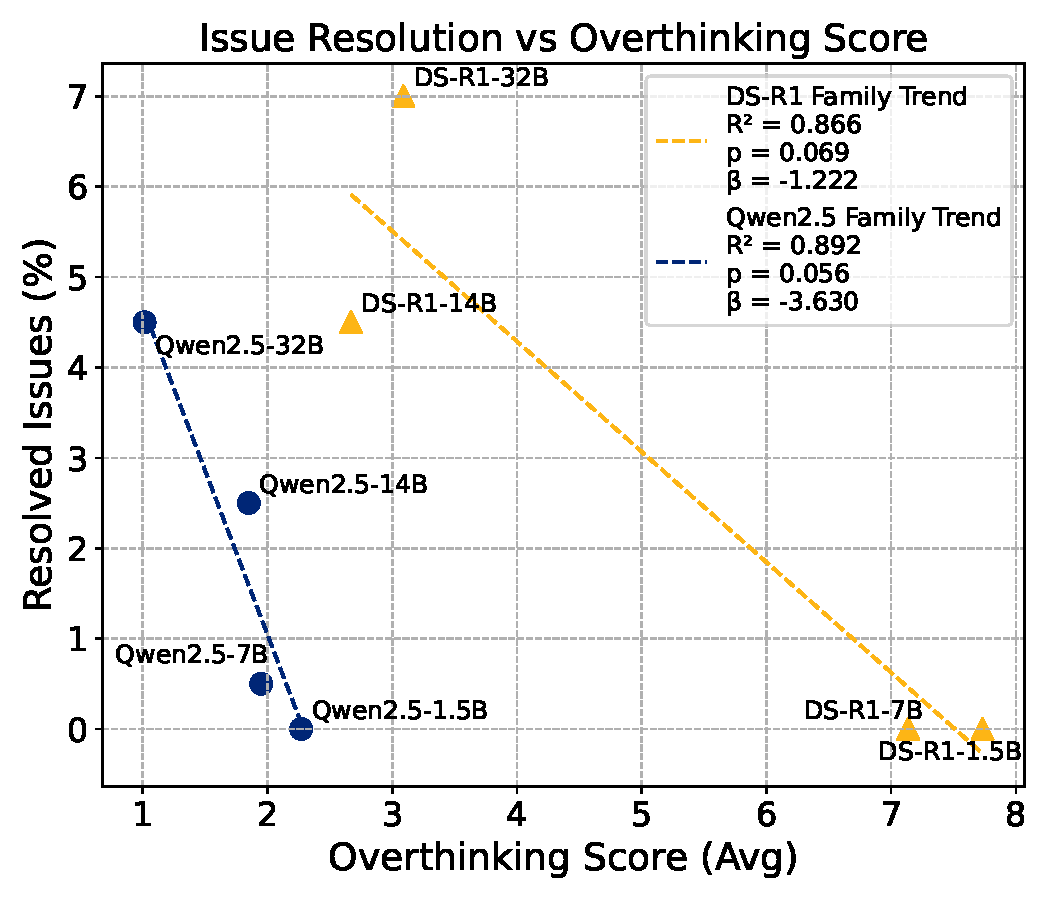
\includegraphics[width=1\linewidth]{size_matters.pdf}
    \caption{This graph showcases that both families show strong negative correlations between overthinking and performance. Both relationships are nearly significant despite small sample sizes. The p-values are close to conventional significance suggesting a trend.}
    \label{fig:figure5}
\end{figure}

As detailed in \cref{tab:overthinking_comparison}, R1 models exhibit significantly higher overthinking scores compared to their Qwen2.5 counterparts, with this gap widening as model size decreases.

\begin{table}[ht]
\centering
\begin{tabular}{lccc}
\bottomrule
\textbf{Measure} & \textbf{Value} \\
\midrule
DS-R1 Family        & 5.157 $\pm$ 2.292 \\
Qwen2.5 Family      & 1.771 $\pm$ 0.463 \\
\midrule
T-test statistic     & 2.508 \\
T-test p-value       & 0.046 \\
\bottomrule
\end{tabular}
\caption{Overthinking Score Comparison for R1 and Qwen2.5}
\label{tab:overthinking_comparison}
\end{table}

\section{Overthinking and Token Usage}
\label{sec:token_usage}

We investigated the relationship between token consumption and overthinking behavior in the o1 model by manipulating the model's reasoning effort parameter between high and low settings. Our analysis revealed that o1 models with low reasoning effort demonstrate 35\% higher overthinking scores compared to their high-effort counterparts.

As shown in \cref{tab:o1_model_comparison}, the difference in averaged overthinking scores between the two configurations is statistically significant, suggesting that increased token allocation might reduce overthinking in agentic contexts.

\begin{table}[ht]
\centering
\begin{tabular}{lc}
\toprule
\textbf{Measure} & \textbf{Value} \\
\midrule
O1 Low        & 3.327 $\pm$ 4.539 \\
O1 High       & 2.467 $\pm$ 4.123 \\
\midrule
T-test p-value & 0.050 \\
\bottomrule
\end{tabular}
\caption{Comparison of o1 Models with Different Reasoning Efforts}
\label{tab:o1_model_comparison}
\end{table}

\section{Overthinking and Context Window}
\label{sec:context_window}

When comparing models of similar size but different context windows—such as DS-R1-32B versus QwQ and GPT-4o-mini versus SkyT1—we found no consistent relationship between context window size and overthinking tendencies. These observations suggest that context window size may not be a primary factor in determining a model's propensity for overthinking.

\section{Practical Implications}
\label{sec:implications}

OpenAI has demonstrated that reasoning models exhibit a disproportionate increase in computational costs relative to their performance gains \cite{arcprize2024oai}. Our experiments with SWE-bench Verified dataset confirm this observation: o1 with high reasoning effort achieves a 29.1\% resolution rate at \$1,400, while the low reasoning variant reaches 21.0\% at \$400—a 3.5x cost difference for an 8.1 percentage point improvement in performance.

To address this efficiency gap, we developed an alternative approach: running the low-reasoning variant twice and selecting traces with minimal overthinking scores. This method achieved a \textit{26.3\% resolution rate while consuming only 57\% of the high-reasoning configuration's cost}, as shown in \cref{fig:figure2}. Our findings suggest that monitoring and controlling overthinking behavior could be a cost-effective strategy for optimizing model performance in real-world applications.